\documentclass[twoside,12pt]{article}
\usepackage{amssymb,amsmath, amsfonts,latexsym,mathtext, array, graphicx, geometry, caption, subcaption, bbm}
\geometry{margin=1.5cm}
\setlength{\parskip}{0.8ex plus 0.1ex minus 0.2ex}
\newcommand{\M}[1]{\boldsymbol{\mathbf{#1}}}
\newcommand{\V}{\M}
\newcommand{\Cal}{\mathcal}
\bibliographystyle{plain}

\newtheorem{thm1}{Theorem}
\newtheorem{def1}{Definition}

\begin{document}

\title{Machine Learning 6.867 - Final Report\\Robust Artificial Neural Networks}
\author{Ying (Daisy) Zhuo}

\maketitle

\begin{abstract}
Artificial neural network is a popular and successful machine learning method. However, when data are subject to uncertainty, the model can be unstable and overfit the training data. In this project, I explored the possibility of immunizing ANNs against uncertainties in data via robust optimization. I derived the robust formulation and established its connection with regularization and adversarial training. As a preliminary computational experiment (but not the focus of the paper), I implemented the method and observe that Robust-ANN offers slightly higher out-of-sample accuracy in the MNIST dataset.

\end{abstract}


\section{Introduction}

Artificial neural networks (ANN) have been shown to have very strong performance for many challenging machine learning tasks such as image recognition and natural language processing. This is largely due to its ability to approximate non-linear functions arbitrarily well and to extract patterns from complicated or noisy data. However, the generalization performance of neural networks can be severely impacted by overfitting the training set. %This project presents a formulation of ANN that is robust to uncertainties in data, and demonstrates the benefits it offers. 

Regularization is classical approach to reduce overfitting in many machine learning methods. By adding a penalty on the weight parameters to the objective function, the weight parameters are shrunk toward zero. Smaller weights give smoother network response and can potentially reduce overfit. One simple regularizer is \emph{weight decay}, which adds a $\lambda \M w ^T \M w$ term to the error function. In a probabilistic view, simple weight decay regularization is equivalent to putting a Gaussian prior over the weight parameters. 

Unfortunately, simple weight decay does not achieve the desirable property of \emph{consistency}, also known as scaling invariance. The invariance property says if we linearly transform the input or target vector, we should obtain equivalent network with linear transformation of weights as given. However, the simple weight decay regularizer term does not maintain this property, as it penalizes on all weights equally. One scale-invariant regularizer is to use different trade-off parameters for the two weights; i.e., adding $\lambda_1 \| \M w^{(1)}\|^2 + \lambda_2 \| \M w^{(2)}\|^2$ to the negative log likelihood, biases excluded. In the Bayesian framework, putting different priors on $\M w^{(1)}$ and $\M w^{(2)}$ corresponds to an improper prior, which cannot be normalized. Using improper priors can lead to difficulty in selecting regularization coefficients and Bayesian model comparisons \cite{bishop2006pattern}.

Given the somewhat ad hoc nature of adding regularizers and difficulty in the Bayesian framework on neural networks, I would like to consider the issue from a different perspective. In a recent paper, Bertsimas et al. proposed a principled approach using robust optimization to model data uncertainty, and have shown its equivalence to regularization in certain circumstances \cite{bertsimas2015robust}. For example, by modeling uncertainty in input features  on hinge-loss minimization, it is equivalent to support vector machines. The computational results in the paper suggest that addressing uncertainties from robust perspective offers better generalization, as demonstrated in logistic regression, support vector machine, and decision trees. The results are encouraging and hint that there is potential improvement via robustification for more complex models such as ANN.

In this project, I first introduce robust optimization at a high level, then derive the formulation of Robust-ANN that can be readily implemented with low incremental computational overhead. I further establish the resemblance between Robust-ANN and regularization, and discuss some of its properties. Since the focus of this paper is more on the theoretical development, I offer limited preliminary computational evidence by testing on the MNIST and compare the performance of between Robust and non-robust ANNs.


\section{Overview of Robust Optimization}

This section is an overview of robust optimization that introduces the notions of uncertainty sets and robust counterparts that will be used later when applying robust optimization techniques to ANN. Some of the content is adapted from \cite{bertsimas2015robust}.

Robust optimization is arguably one of the fastest growing areas in optimization in the past decade. As a means for modeling uncertainty in optimization problems without the use of probability distributions, it is demonstrated to be both computationally tractable and offer attractive solutions.

Under this modeling framework, we construct deterministic \emph{uncertainty sets} that contain possible values of uncertain parameters. We then seek a solution that is optimal for all such realizations of this uncertainty. Consider the general optimization problem:
\[
\begin{aligned}
  \max_{\V x \in \Cal X} ~~ & c(\V u, \V x)\\
  \textup{s.t.} ~~ & \V g (\V u, \V x) \le 0.
\end{aligned}
\]
where $\V x$ is the vector of decision variables, and $\V u$ is a vector of given parameters. Relaxing the assumption that $\V u$ is fixed, we assume instead that the realized values of $\V u$ are restricted to be within some uncertainty set $\Cal U$. We form the corresponding robust optimization problem by optimizing against the worst-case realization of the uncertain parameters across the entire uncertainty set:
\[
\begin{aligned}
  \max_{\V x \in \Cal X} ~~ & \min_{\V u \in \Cal U} \; c(\V u, \V x) \\
  \textup{s.t.} ~~ & \V g (\V u, \V x) \le 0 ~~ \forall \V u \in \Cal U.
\end{aligned}
\]
Despite typically having an infinite number of constraints, it is often possible to reformulate the problem as a deterministic optimization problem with finite size, depending on the choice of uncertainty set $\Cal U$. The resulting deterministic problem is deemed the \emph{robust counterpart}, which is generally a problem of the same complexity as the nominal problem.


There is extensive evidence in the literature that robust solutions have significant advantages relative to nominal solutions. In essence, we are willing to accept robust solutions that are suboptimal in the nominal case under the data at hand, but are much more often feasible/optimal when data are perturbed. In the case of machine learning problem, such trade-off is especially important to avoid overfitting the training data.

\section{Theoretical Derivation}

The derivation in this section is conducted independently of \cite{shaham2015understanding}. 
Let $E(\M x^{(i)}, \M y^{(i)}, \M w)$ be the negative log likelihood of single training data point $( \M x^{(i)}, \M y^{(i)} )$ in an ANN. Thus, the optimization problem to be solved is
\begin{equation}
\min_{\M w} ~ \sum_{i=1}^n E(\M x^{(i)}, \M y^{(i)}, \M w)
\end{equation}

Under a given uncetainty set $\Cal U$ on data $\M x$, the robust formulation of ANN is then:
\begin{equation}\label{eq:RANN}
\min_{\M w} ~ \max_{\Delta \M x \in \Cal U}~  \sum_{i=1}^n E(\M x^{(i)} + \Delta \M x^{(i)}, \M y^{(i)}, \M w)
\end{equation}

The exact robust counterpart for Problem \eqref{eq:RANN} cannot be readily obtained, due to the complex non-linear and non-convex structure of the objective function. However, with some assumptions and a little machinery, we can approximate the original problem while keeping the problem at the same level of computational complexity as the nominal one. To simplify the problem a bit, let's assume $\Cal U$ decouples across the data points. For example, a common uncertainty set can be constructed as $\| \M x^{(i)} \|_p \leq \rho$ for each $i$. This way, the inner minimization is separable among the $i$'s; i.e., we need to solve for 
\begin{equation}\label{eq:RANN_inner}
\max_{\Delta \M x^{(i)}}  E(\M x^{(i)} + \Delta \M x^{(i)}, \M y^{(i)}, \M w)
\end{equation}

for each $i$. As demonstrated in \cite{bertsimas2015robust}, the particular choice of uncertainty set does not affect the improvement drastically for many classifiers, therefore this choice is warranted.

To solve Problem \eqref{eq:RANN_inner}, we consider a Taylor first-order expansion:
\begin{equation}\label{eq:RANN_taylor}
E(\M x^{(i)} + \Delta \M x^{(i)}, \M y^{(i)}, \M w) = E(\M x^{(i)}, \M y^{(i)}, \M w) + \nabla_{\M x} E(\M x^{(i)}, \M y^{(i)}, \M w) ^T \Delta \M x^{(i)}
\end{equation}

When $\Cal U = \{\| \M x^{(i)} \|_\infty \leq \rho \}$ (i.e., $\max_r |\M x_r^{(i)}| \leq \rho$), the minimizer $\Delta \M x^{(i)}$ should take on value of $\rho \cdot sign(\nabla_{\M x} E(\M x^{(i)}, \M y^{(i)}, \M w))$ component-wise. Substituting to the objective gives
\begin{equation*}\label{eq:RANN_inner_linf}
\max_{\Delta \M x^{(i)}}  E(\M x^{(i)} + \Delta \M x^{(i)}, \M y^{(i)}, \M w) = E(\M x^{(i)}, \M y^{(i)}, \M w) + \rho \| \nabla_{\M x} E(\M x^{(i)}, \M y^{(i)}, \M w) \|_1
\end{equation*}

Similarly, when $\Cal U = \{\| \Delta \M x^{(i)} \|_1 \leq \rho \}$ (i.e., $\sum_{i=1}^n |x_r^{(i)}| \leq \rho$), at optimality $\Delta \M x_r^{(i)}$ takes on $\rho$ at the component with the largest value of $\nabla_{\M x} E(\M x^{(i)}, \M y^{(i)}, \M w)$, and zero at all other components. Substituting to the objective gives
\begin{equation*}\label{eq:RANN_inner_l1}
\max_{\Delta \M x^{(i)}}  E(\M x^{(i)} + \Delta \M x^{(i)}, \M y^{(i)}, \M w) = E(\M x^{(i)}, \M y^{(i)}, \M w) + \rho \| \nabla_{\M x} E(\M x^{(i)}, \M y^{(i)}, \M w) \|_\infty
\end{equation*}

To summarize, Problem \eqref{eq:RANN} can be reformulated as follows:
\begin{equation}\label{eq:RANN_rc}
\min_{\M w} \sum_{i=1}^n \left[E(\M x^{(i)}, \M y^{(i)}, \M w) + \rho \| \nabla_{\M x} E(\M x^{(i)}, \M y^{(i)}, \M w) \|_{p^*}\right],
\end{equation}

where $\|\cdot \|_p^*$ is the dual norm of $\|\cdot \|_p$ (i.e., $1/p + 1/p^* = 1$).

The approximate robust counterpart problem in \eqref{eq:RANN_rc} can be solved efficiently using numeric optimization methods, if the gradient of the second term can be expressed explicitly. Compared to a regularized ANN (two-layer network for example):
\begin{equation*}
\min_{\M w} \sum_{i=1}^n \left[E(\M x^{(i)}, \M y^{(i)}, \M w)\right] + \lambda_1 \| \M w^{(1)}\|^2 + \lambda_2 \| \M w^{(2)}\|^2,
\end{equation*}
 
Robust-ANN adds to the objective a single penalization term that depends on the gradient (which in turn depends on the weights at all levels). Formulation \eqref{eq:RANN_rc} has advantage as it has a stronger theoretical basis rooted in robustness, contains fewer parameters to cross-validate, and avoids the issue of improper prior.
 
In practice, one can solve the robust formulation in \eqref{eq:RANN_rc} without writing the gradient explicitly. An iterative method is proposed as follows: first fix initial $\M w$ and find the most adversarial $\Delta \M x_i$ for each $i$ based on $\nabla_{\M x} E(\M x^{(i)}, \M y^{(i)}, \M w)$. Then one can update the $\M x_i$ and run a basic ANN forward-backward procedure to obtain $\M w$. The algorithm terimnates when $\M w$ converges. A more efficient method, proposed in \cite{shaham2015understanding}, takes a single descent step to update $\M w$ under the perturbed data rather than solving each substep to optimality. Under this, the training time is about twice as long as basic ANN.


\section{Implementation and Computational Results}
I implemented Robust-ANN in the programming language \textsf{Julia} with package \textsf{MXNet}, an efficient and flexible deep learning framework \cite{mxnet}. I chose to use this package rather than writing my own from scratch in order to take advantage of the computational efficiency and to obtain a decent baseline to compare with. To benchmark, the implementation is tested on the MNIST dataset of handwritten digits, with $50,000$ data points in training, $10,000$ in evaluation, each of dimension $784$ ($28 \times 28$ pixels). The outputs are digits $0$ through $9$. The network structure has three layers and is presented in Figure~\ref{fig:ann_arc}. Other model specifications include: number of epoch is 3 to ensure baseline method obtains decent accuracy, learning rate is 0.1, momentum is 0.9, weight decay coefficient is $10^{-5}$. We use a stochastic gradient descent optimizer, with batch size being 100. Since the problem size is small, we only use CPU for this purpose. To ensure the randomness in initialization does not affect the comparison, we set the same seed in both cases.

\begin{figure}[ht!]
    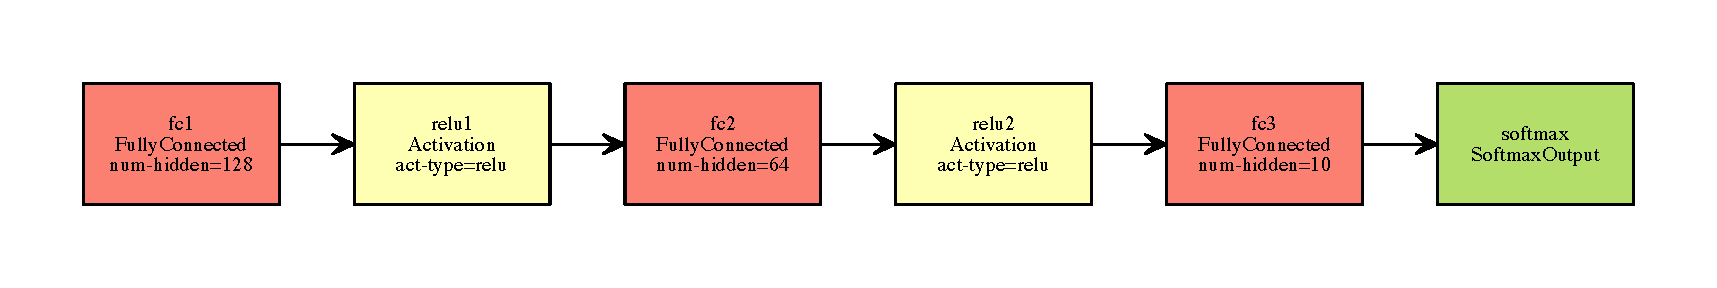
\includegraphics[scale=0.7]{visualize.pdf}
    \caption{Illustration of ANN architecture in computational experiments.}
    \label{fig:ann_arc}
\end{figure}

The procedure of Robust-ANN is as follows: after an iteration of basic ANN, a back-propagation is called on each small batch to obtain the gradients, which in turn is used to calculate the adversarial perturbation $\Delta \M x_i$. A small complication is that \textsf{MXNet} does not provide gradient with respect to the data $\M x^{(i)}$ directly; to obtain such, we take the current first level weights $\M w$, the gradient with respect to the ReLU activation $\frac{\partial J}{\partial \M a}$ and do the following calculation:


\begin{equation}
\begin{aligned}
\frac{\partial J}{\partial \M x} 
& = \sum_{j=1}^{n_1} \frac{\partial J}{\partial a_j} h'(\M w_j^T \M x) \M w_j\\
& = \sum_{j=1}^{n_1} \frac{\partial J}{\partial a_j} \mathbbm{1}_{\{\M w_j^T \M x > 0 \} } \M w_j
\end{aligned}
\end{equation}

The gradient of the activation function (ReLU here) can easily be adapt to that of logistic function or tanh. Depending on the choice of uncertainty set, we can construct different adversarial $\Delta \M x^{(i)}$. In this example, we consider the $l_\infty$ norm uncertainty set and therefore obtain $\M x_i^{\textrm{new}} = \M x_i^{\textrm{old}} + \rho * sign(\frac{\partial J}{\partial \M x})$. We can now fit the a new basic ANN with the updated $\M x_i^{\textrm{new}}$ until convergence. The convergence is measured as the negative log likelihood being no farther than 1 between iterations.

We obtain the following preliminary results: the base case ANN achieves an out-of-sample accuracy of $96.94\%$. Robust-ANN converges after 15 iterations and achieves an out-of-sample accuracy of $97.27\%$. To compare, robustness offers a slight improvement of $0.33\%$. 


\section{Conclusions}
In this project, I explore the possibility of adding robustness against uncertainties in data. I implemented Robust-ANN and observe that it offers slightly higher out-of-sample accuracy in the MNIST dataset. Whether this improvement is significant needs further testing on other datasets and various other specifications of the model. Regardless, the paper presents a formulation of ANN that offers robustness to uncertainties in principle, and may demonstrate better out-of-sample performance.


\bibliography{ref}

\end{document}